\documentclass[12 pt]{article}
\usepackage[margin = 1cm]{geometry}
\usepackage [utf8]{inputenc}
\usepackage[T2A]{fontenc}
\usepackage[russian]{babel}
\usepackage{dsfont }
\usepackage{hyperref} 
\usepackage{graphicx}
\usepackage{amsthm, amsmath, amssymb}
\usepackage{xcolor}

\begin{document}

{\bf \Large Motivation} \\

As the amount of produced libraries, APIs and tools grow dramatically the developers want to reuse them rather than create their own solutions. The fact that such resources as StackOverflow are so popular only proves it.
While the most popular questions are covered by these resources, there are still queries that were not answered. It may take from hours to months for a new question to be answered. Also such resources can’t help with questions about proprietary libraries. That’s why it is necessary to build automatic code search. The labeling of query-code relevance could help to build such a search. \\

You will be given the pairs of a natural language query and a function or method. You need to label how relevant would be this function or method as the result from search system for the query. \\

Through the annotations, we want to measure how relevant would these results be to you. 

\begin{itemize}
	\item You don't have to be absolutely certain about the correctness of the code.
	\item You might be interested in copy-pasting the code, finding a library to use or just getting some understanding about how something is implemented.
	\item You might be searching within your project (e.g. to reuse code witin your project), your company or all of GitHub.
\end{itemize}

{\bf \Large Instruction for query-function relevance labeling. }  \\

If you are {\bf not} provided with the account credentials:
\begin{itemize}
	\item Register on \href{https://labelbox.com}{Labelbox}
	\item Send account's e-mail to the @belatriss (telegram). 
	\item Wait until you are added as a labeler to the project.
	\item You get an e-mail with the invitation to switch the organisation, do it.
	\item Go to the projects page -- there should apper the project "Query code relevance".
	\item Start labeling. Label $\sim$ 150-200 pairs. The more pairs you label, the better.
\end{itemize}

If you are provided with the account credentials:
\begin{itemize}
	\item Log in \href{https://labelbox.com}{Labelbox}
	\item Go to the projects page -- there should apper the project "Query code relevance".
	\item Start labeling. Label $\sim$ 150-200 pairs. The more pairs you label, the better.
\end{itemize}


{\bf \Large Instruction for labeling. } 

Please annotate the results according to the following scheme:
\begin{itemize}
	\item {\bf 3: Exact match.} This seems exactly what was looking for. I would copy-paste the code and make minor adaptations or will use this functionality of the library in my code. 

	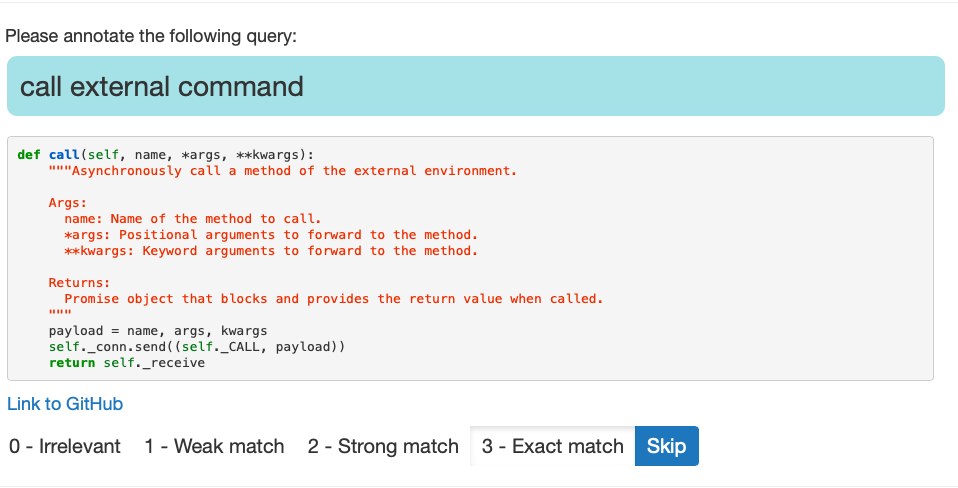
\includegraphics[width=\textwidth]{exact_match.png}
	\includegraphics[width=\textwidth]{exact_match_2.png}
	\item {\bf 2: Strong match.} This does more or less what I was looking for. I would use the code in here as a backbone for my purpose, but I won't necessarily copy-paste it or use this library.

	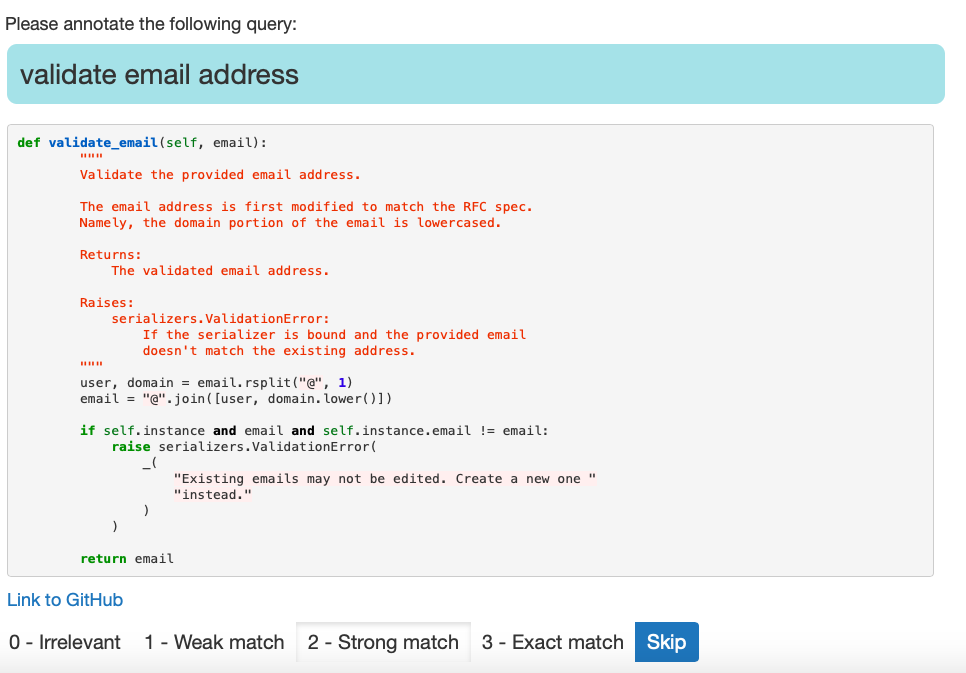
\includegraphics[width=\textwidth]{strong_match}
	\includegraphics[width=\textwidth]{strong_match_2.png}
	\item {\bf 1: Weak match.} That's not exactly what I was looking for, but there are some useful elements/pointers to things that I would use (e.g. APIs, code structure) and can form the basis of a new query or exploration towards solving my query.

	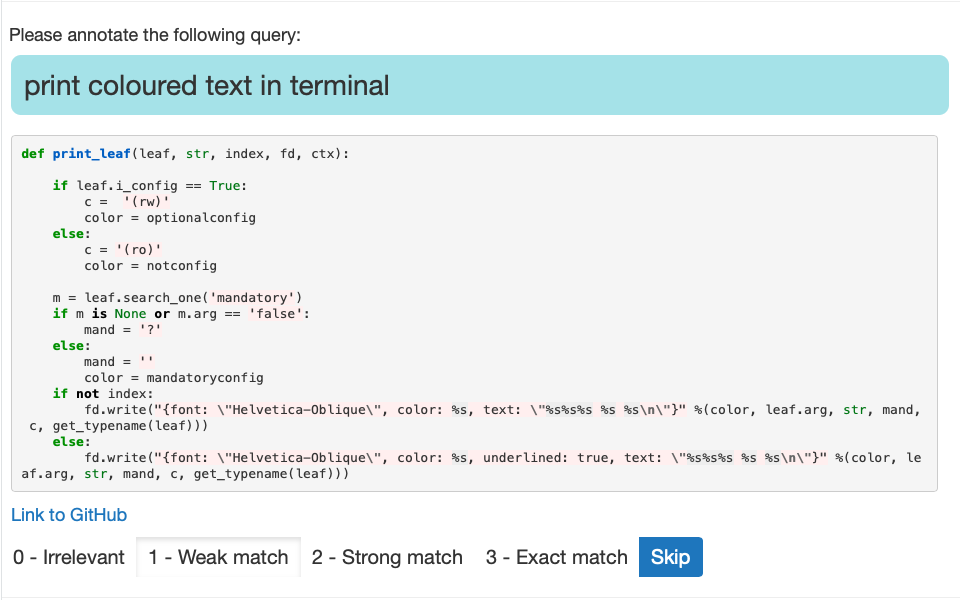
\includegraphics[width=\textwidth]{weak_match}
	\item {\bf 0: Irrelevant.} I would never want to see this tor this query.
	
	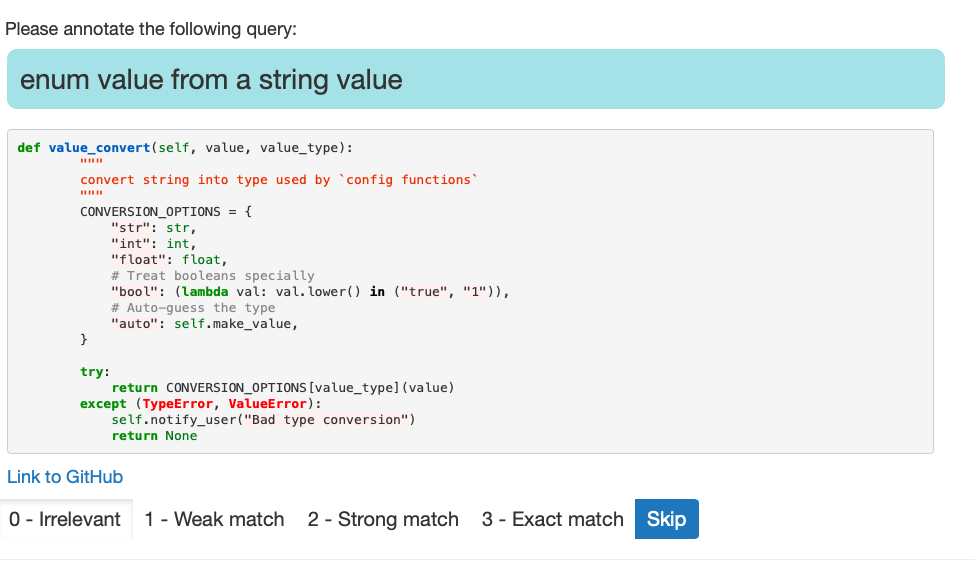
\includegraphics[width=\textwidth]{irrelevant}
\end{itemize}

\end{document}